\documentclass{article}
\usepackage[utf8]{inputenc}
\usepackage{amsmath}
\usepackage{amsfonts}
\usepackage{tikz}
\usepackage{tkz-euclide}
\usepackage{graphicx}
\graphicspath{ {./images/} }
\pagenumbering{gobble}

\begin{document}

\begin{center}
        \section*{Maths Problems Set 6 (23 June 2020)}
\end{center}

\begin{enumerate}

    \item %1
    A father is twice the age of his son, and the digits of the son's age are the digits of the father's age reversed. What age is the father?
    
    
    \item
    There are three jars, one with red fruit, one with blue fruit and one with red and blue fruit. You can’t see inside the jars. Ammar has mischievously relabelled the jars, but foolishly he tells you that each label is on the wrong jar. Provide a strategy such that you can correctly relabel the jars by checking a random fruit from a jar of your choice.
    
    \item
    There are 100 ants on a 99 meter long rod, distributed on the rod such that there is a distance of 1 meter between each ant and each ant is facing towards the center of the rod. The ants move with a constant speed of 1 metre every 10 seconds and they change direction upon collision with one another. How long until all the ants have fallen off the rod and how many collisions will there have been?
    
    \item
    What is the maximum possible area of a triangle whose perimeter has length $p$?
    
    \item
    Andrew, Bruce, Chloe, and David are sitting in a circle playing a passing game where on any given turn the player with the parcel passes the parcel to the left $25\%$ of the time, to the right $25\%$ of the time, and they hold onto it $50\%$ of the time. Given that Andrew starts with the parcel, find the probability for each player of having the parcel on the n-th turn.
    
    \item
    For an integer $n > 1$, prove that $n^4 + 4^n$ is not prime.
    
    \item Find the area shaded in red.\\ % 6-8
    \\
    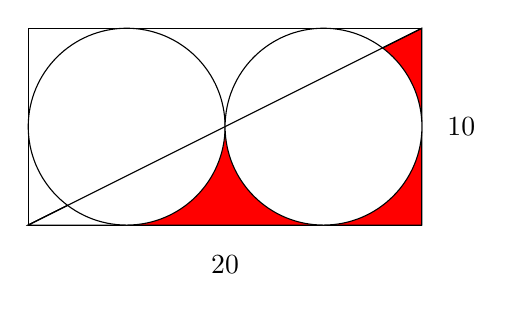
\begin{tikzpicture}[scale=0.25]
        \draw[fill=red!100] plot[smooth, samples=100, domain=20:0] (\x,0.5 * \x) -| (20,10) -- cycle;
        \draw[fill=white!100] plot[smooth, samples=100, domain=5:0] (\x,0.5 * \x) -| (5,0) -- cycle;
    
        \draw (0,0) -- (20,0) -- (20,10) -- (0,10) -- cycle;
        
        \draw[fill=white] (5, 5) circle [radius=5];
        \draw[fill=white] (15, 5) circle [radius=5];
        \draw (0,0) -- (20,10);
        
        \node[label] at (10, -2) {20};
        \node[label] at (22, 5) {10};
        
        
    \end{tikzpicture}

    % Fairly hard. Late page 1
	\item
	Consider a set of lattice points. For what n can a regular convex n-gon sit atop the lattice points such that each vertex of the shape lives on a lattice point?
    
    \item Let $G$ be a convex quadrilateral. Show that there is a point $X$ on the plane of $G$ with the property that every straight line through $X$ divides $G$ into two regions of equal area if and only if $G$ is a parallelogram.

    % Integral evaluation fairly hard
	\item
	Evaluate the following integrals:
	\begin{enumerate}
	    \item $\int \sin^{n}(x) dx$
	    \item $\int \cos^{n}(x) dx$
	    \item $\int \dfrac{1}{1 - \sin(x)}dx$
	    \item $\int\limits_{0}^{\pi}\dfrac{x^{2}\sin(x)}{3 + \sin^2(x)}dx$
	\end{enumerate}

    % Diff equation fairly hard
	\item
	Find the general solution to the following differential equations:
	\begin{enumerate}
	    \item $\dfrac{d^{3}y}{dx^{3}} - 3\dfrac{d^{2}y}{dx^{2}} + 4y = 0$\\
	    \item $\dfrac{d^{4}y}{dx^{4}} + 4\dfrac{d^{3}y}{dx^{3}} + 6\dfrac{d^{2}y}{dx^{2}} + 4\dfrac{dy}{dx} + y = 0$\\
	    \item $(4x+1)\dfrac{d^{2}y}{dx^{2}}+2x\dfrac{dy}{dx}-y=(x+1)^{2}$
	\end{enumerate}


    \item
    Two particles $X$ and $Y$ of equal mass $m$ lie on a smooth horizontal table and are connected by a light elastic spring of natural length $a$ and modulus of elasticity $\lambda$. Two more springs, identical to the first, connect $X$ to a point $P$ on the table and $Y$ to a point $Q$ on the table. The distance between $P$ and $Q$ is $3a$. Initially, the particles are held so that $XP = $, $YQ = $, and $PXYQ$ is a straight line. The particles are then released.
    
    Find the positions of particles $X$ and $Y$ in terms of the time since their release.

    \item
    Suppose we have a floor made of parallel strips of wood, each the same width, and we drop a needle onto the floor. What is the probability that the needle will lie across a line between two strips?

    \item
    Alice and Barbara play a game with a pack of $2n$ cards, each of which has a positive integer written on it. The pack is shuffled and the cards laid out in a row, with the numbers facing upwards. Alice starts, and the players take turns to remove one card from either end of the row, until Barbara picks up the final card. Each player’s score is the sum of the numbers on her chosen cards at the end of the game. Prove that Alice can always obtain a score at least as great as Barbara’s.
    
    
    
    
    
    
    
    
    % Gilad's chess problem
    % \item
    
    % Green eyed dragon problem
    % \item
    % You visit a remote desert island inhabited by one hundred very friendly dragons,all of whom have green eyes. They haven’t seen a human for many centuries and are very excited about your visit. They show you around their island and tell you all about their dragon way of life (dragons can talk, of course).They seem to be quite normal, as far as dragons go, but then you find out something rather odd. They have a rule on the island that states that if a dragon ever finds out that he/she has green eyes, then at precisely midnight at the end of the day of this discovery, he/she must relinquish all dragon powers and transform into a long-tailed sparrow. However, there are no mirrors on the island, and the dragons never talk about eye color, so they have been living in blissful ignorance throughout the ages.Upon your departure, all the dragons get together to see you off, and in a tearful farewell you thank them for being such hospitable dragons. You then decide to tell them something that they all already know (for each can see the colors of the eyes of all the other dragons): You tell them all that at least one of them has green eyes.Then you leave, not thinking of the consequences (if any). Assuming that the dragons are (of course) infallibly logical, what happens? If something interesting does happen, what exactly is the new information you gave the dragons?

\end{enumerate}

\end{document}

